\subsection{PCA}
EL primer modelo utilizado para intentar clasificar los datos será el de Analisis de Componentes Principales. Para ello utilizamremos dos algoritmos basados en aprendisaje Hebbiano y reduciremos las instancias de entrenamiento a 3 dimenciones. Lo que esperamos observar es que aquellas instancias que pertenecen a una misma clase de empresa se encuentran cercas unas de otras, pudiendo observar \"nuves\" de puntos bien definidas.

\subsubsection{Implementación}

En particular los algoritmos utilizados serán los de $Oja$ y $Sanger$. Teniendo una complegidad computacional identica y siendo los algoritmos muy similares, lo distintivo entre estos dos metodos es que $Sanger$ ordenará las componentes prinsipales de mayor a menor de acuerdo a sus autovalores mientras que $Oja$ no.

El pseodocodigo utilizado para aprendisaje del algoritmo $Oja$ será:

\begin{algorithm}
\begin{algorithmic}[1]\parskip=1mm
 \caption{ Algoritmo De Oja}
 \STATE{Para toda instancia de entrenamiento, x}
 \STATE{\quad $y = x.W$}
 \STATE{\quad $\tilde x = y.W^T$}
 \STATE{\quad $\Delta W = learning\_rate ((x - \tilde x)^T . y$}
\end{algorithmic}
\end{algorithm}

Mientras que el de $Sanger$

\begin{algorithm}
\begin{algorithmic}[1]\parskip=1mm
 \caption{ Algoritmo De Sanger}
 \STATE{U = Matriz Triangular Superior Con 1s}
 \STATE{Para toda instancia de entrenamiento, x}
 \STATE{\quad $y = x.W$}
 \STATE{\quad $\tilde x = W(y^T.U)$}
 \STATE{\quad $\Delta W = learning\_rate ((x^T - \tilde x) . y$}
\end{algorithmic}
\end{algorithm}

Utilizando el paquete numpy de python es posible traducir este codigo de manera casi exacta y de esa manera aprovechar las optimizaciones matriciales que se realizan sobre los datos.

\subsubsection{Experimentación}

La metodología de experimentación para este tipo de red será:
Primero la entrenaremos con parte del set de datos que nos fue entregado y una vez realizado esto graficaremos los mismo en el espacio marcando con colores cual era la categoría real de cada punto. De esta manera esperamos distinguir nubes de puntos de un mismo color cercanos entre ellos y alejados de aquellos que pertenecen a otras categorías. Como primera instancia quisimos ver que el algormitmo convería realmente a una solución y la manera en que lo realizaba. En el siguiente apartado presentaremos como convergió la solución en cada caso para valores que a priori daban resultados aceptables.

\subsubsection{Sanger}

Utilizando learning rate igual a $0.1$ y $100$ epocas, y una matriz inicial de pesos normal con media 0 y varianza $1/\sqrt(cantidad_neuronas_entrada)$ entrenamos la red y graficamos los resultados intermedios para $0\%,25\%, 50\%, 75\%$ y $100\%$ del entrenamiento. En primer instancia la red comienza completamente desordenada:

\begin{figure}[h!]
\centering
  \centering
  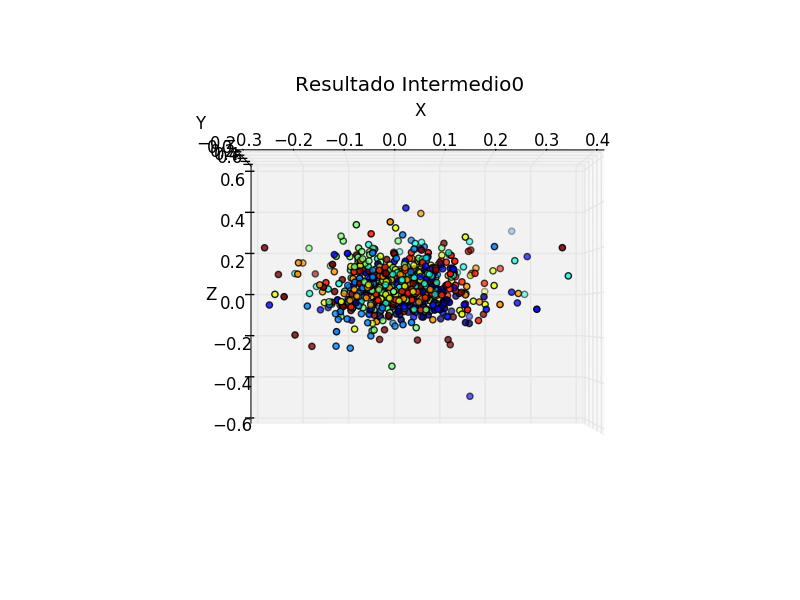
\includegraphics[width=.6\linewidth]{convergencia_oja/0.png}
\caption{Sin entrenar}
\label{fig:test}
\end{figure}


\pagebreak

Luego de $25$ epocas se empieza a observar sierto grado de ordenamiento, por ejemplo, la nube de puntos verdes arriba a la derecha resulta distintiba, lo mismo que una gran agrupación de puntos azules en el medio del grafico.

\begin{figure}[h!]
  \centering
  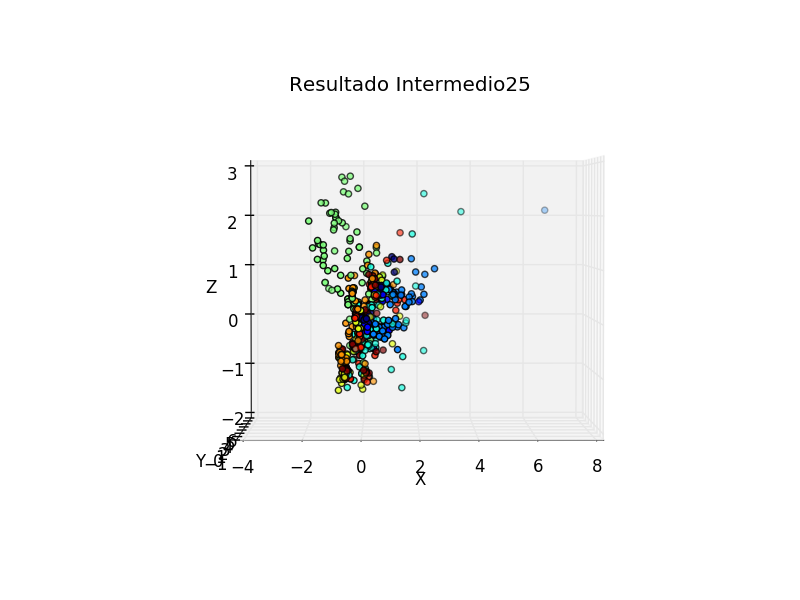
\includegraphics[width=.6\linewidth]{convergencia_oja/1.png}
\caption{25 epocas}
\label{fig:test}
\end{figure}


\pagebreak

Para 50 y 75 epocas continua observandose la convergencia del algoritmo, puede observarse como de alguna manera los clusters de puntos rotan en cierta manera quedando distribuidos de manera mas distinitba en el eje $x$.

\begin{figure}[h!]
\centering
\begin{subfigure}{.5\textwidth}
  \centering
  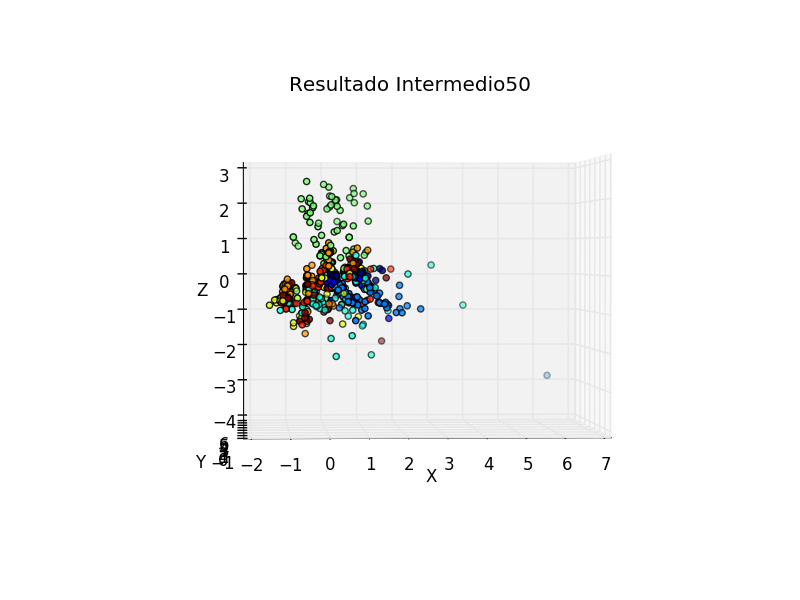
\includegraphics[width=.9\linewidth]{convergencia_oja/2.png}
  \caption{50 epocas}
  \label{fig:sub1}
\end{subfigure}%
\begin{subfigure}{.5\textwidth}
  \centering
  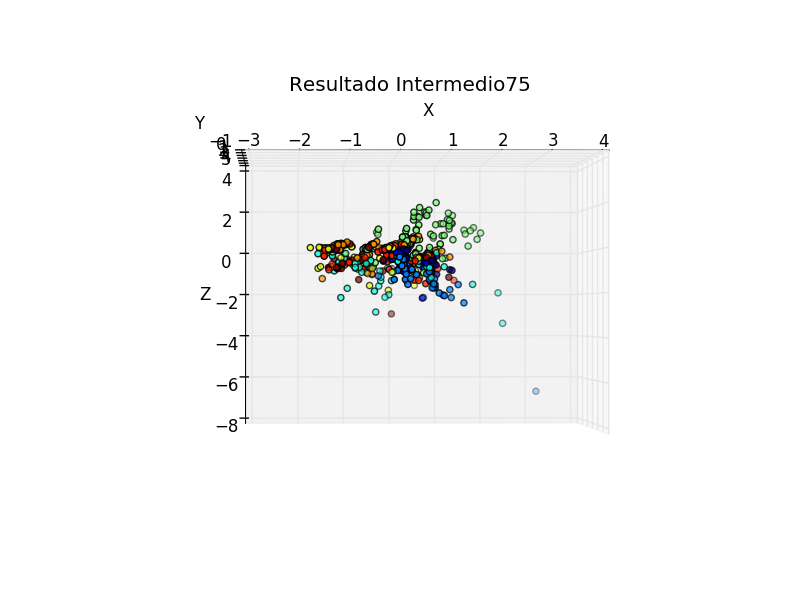
\includegraphics[width=.9\linewidth]{convergencia_oja/3.png}
  \caption{75 epocas}
  \label{fig:sub2}
\end{subfigure}
\caption{50 y 75 epocas}
\label{fig:test}
\end{figure}

Finalmente para $100$ epocas puede verse un alto grado de observación de los puntos. De aqui tambien puede observarse que las 3 componentes principales presentan un grado similar de varianza, estando los datos agrupados en $(-2,2), (-1,3) y (-2,2)$ en $x,y,z$ respectivamente. Ademas el punto con $z=-8$ puede obesrvarse un marcado outlier.

\begin{figure}[h!]
	\centering
	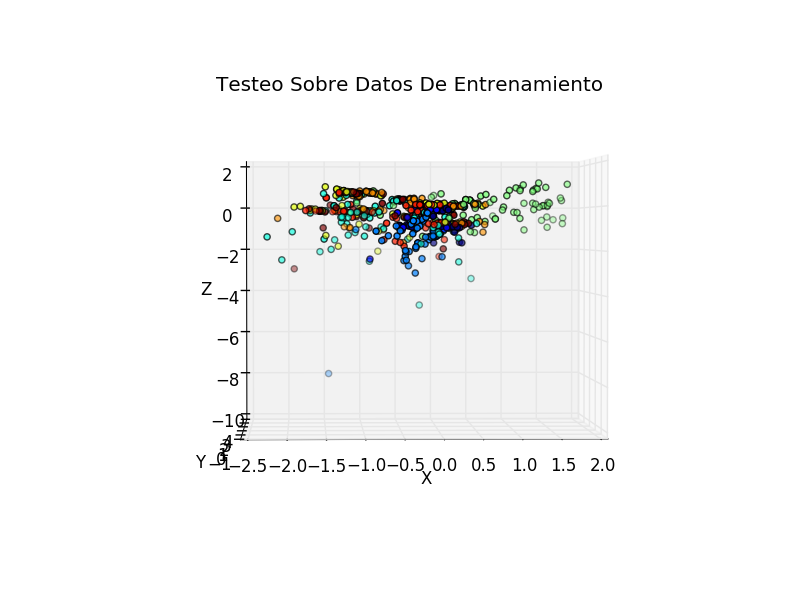
\includegraphics[width=.6\linewidth]{convergencia_oja/4.png}
	\captionof{figure}{100 epocas}
	\label{fig:test1}
	\centering
\end{figure}

\begin{figure}[h!]
  \centering
  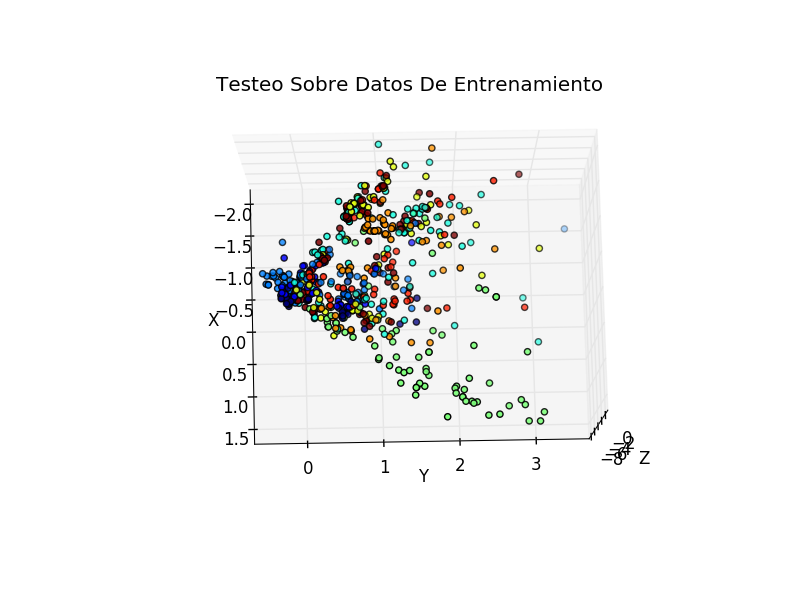
\includegraphics[width=.6\linewidth]{convergencia_oja/42.png}
  \captionof{figure}{100 epocas}
  \label{fig:test1}
  \centering
\end{figure}

\pagebreak

\subsection{Sanger}

Realizando un prodecimiento similar para el algormitmo de sanger, podemos observar los siguentes resultados:

\begin{figure}[h!]
  \centering
  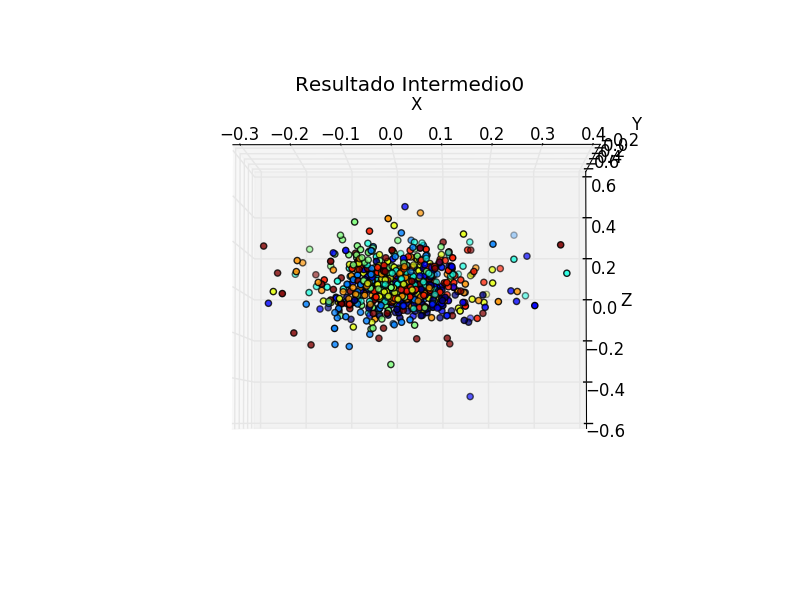
\includegraphics[width=.6\linewidth]{convergencia_sanger/0.png}
\caption{0 epocas}
\label{fig:test}
\end{figure}

\pagebreak

Comenzando sin ningun tipo de ordenamiento en los datos.

\begin{figure}[h!]
  \centering
  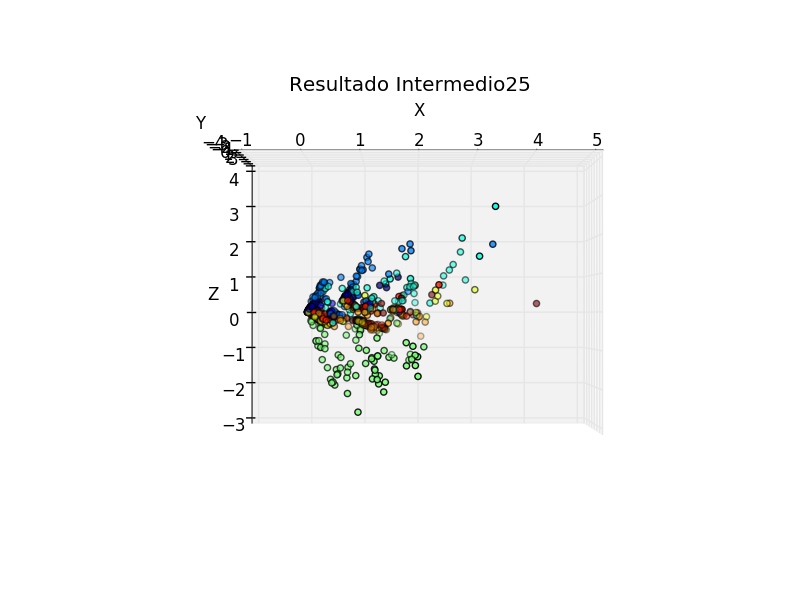
\includegraphics[width=.6\linewidth]{convergencia_sanger/1.png}
\caption{25 epocas}
\label{fig:test}
\end{figure}

Aqui ya puede observarse nuevamente sierto ordenamiento de los datos.

\begin{figure}[h!]
\centering
\begin{subfigure}{.5\textwidth}
  \centering
  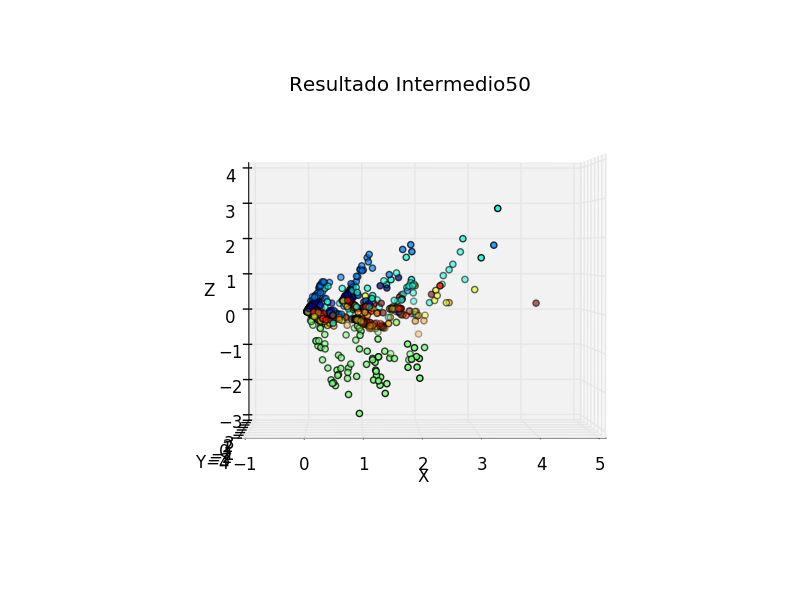
\includegraphics[width=.4\linewidth]{convergencia_sanger/2.png}
  \caption{50 epocas}
  \label{fig:sub1}
\end{subfigure}%
\begin{subfigure}{.5\textwidth}
  \centering
  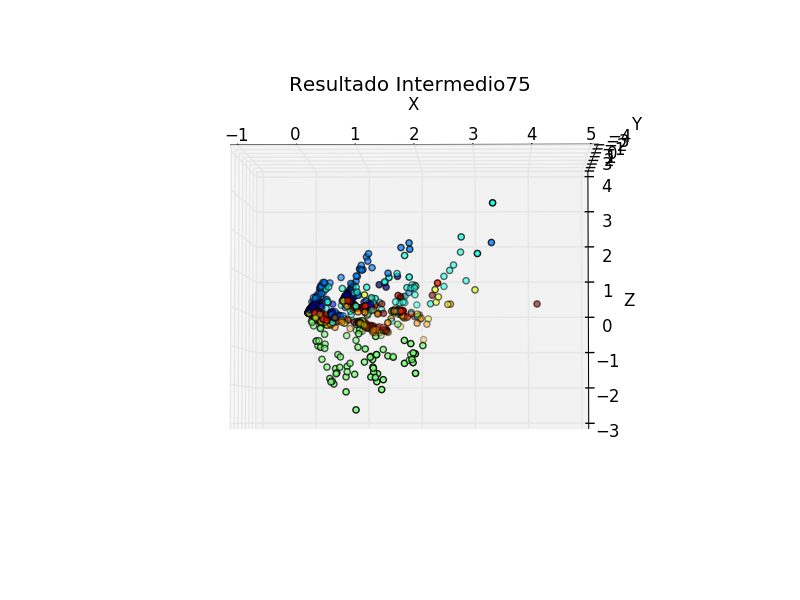
\includegraphics[width=.4\linewidth]{convergencia_sanger/3.png}
  \caption{75 epocas}
  \label{fig:sub2}
\end{subfigure}
\caption{Resultados Intermedios}
\label{fig:test}
\end{figure}

\begin{figure}[h!]
	\centering
	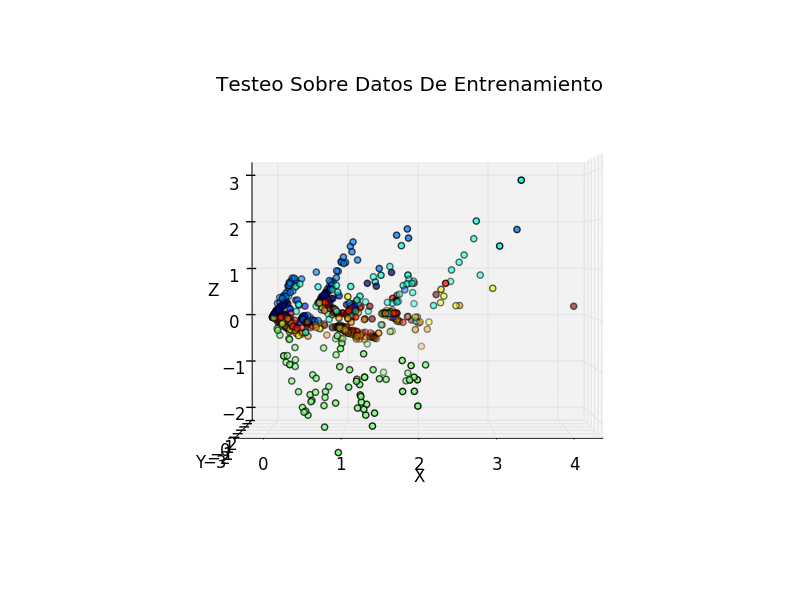
\includegraphics[width=.6\linewidth]{convergencia_sanger/4.png}
  %\captionof{figure}{100 epocas}
  \label{fig:test1}
  \centering
  \caption{100 epocas}
\end{figure}

Nuevamente encontramos aqui nuevamente los datos ordenados 

%Neural Networks Haykin
% In Chatterjee et al. (1998), the convergence properties of the GHA algorithm
% described in Eq. (8.91) are investigated. The analysis presented therein shows that
% increasing  leads to faster convergence and larger asymptotic mean-square error, which
% is intuitively satisfying. In that paper, the tradeoff between the accuracy of computation
% and speed of learning is made explicit.

\subsection{Overfiting en Sanger y Oja}

La proxima experimentación que realizaremos será ver que grado de overfiting realizan estos algoritmos sobre los datos de entrenamiento. Para eso entrenamos con una porción de los datos y utilizaremos el resto para ver graficamente la calidad de los resultados:

\begin{figure}[h!]
\hspace{-2cm}\begin{minipage}{.7\textwidth}
  \centering
  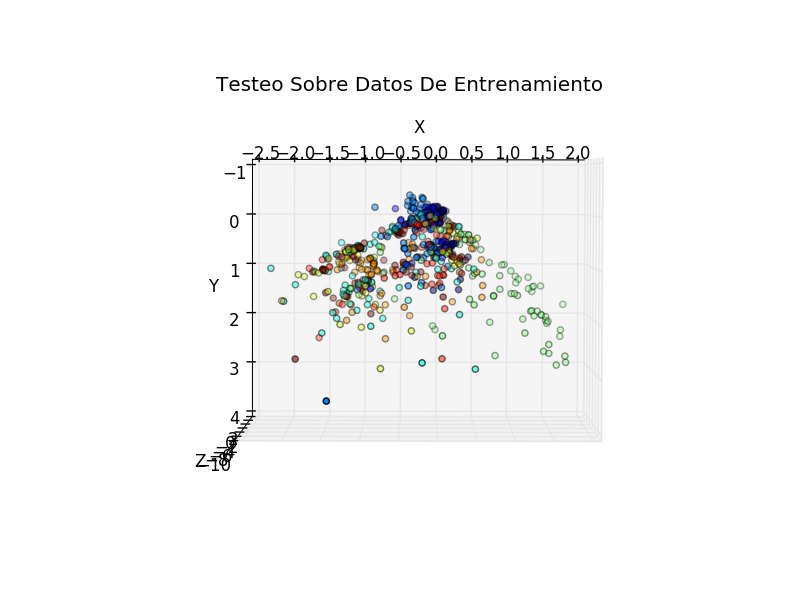
\includegraphics[width=.9\linewidth]{testeo_test_set_oja/entrenamiento12.png}
  \captionof{figure}{Datos Entrenamiento}
  \label{fig:test1}
\end{minipage}%
\hspace{-3cm}
\begin{minipage}{.7\textwidth}
  \centering
  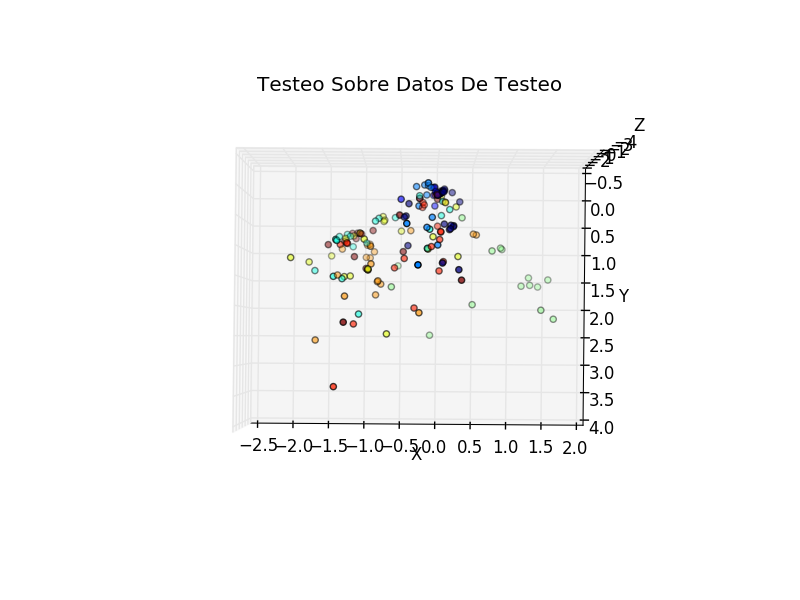
\includegraphics[width=.9\linewidth]{testeo_test_set_oja/test_12.png}
  \captionof{figure}{Datos Testeo}
  \label{fig:test2}
\end{minipage}
\captionof{figure}{Oja}
\end{figure}


\begin{figure}[h!]
\hspace{-2cm}\begin{minipage}{.7\textwidth}
  \centering
  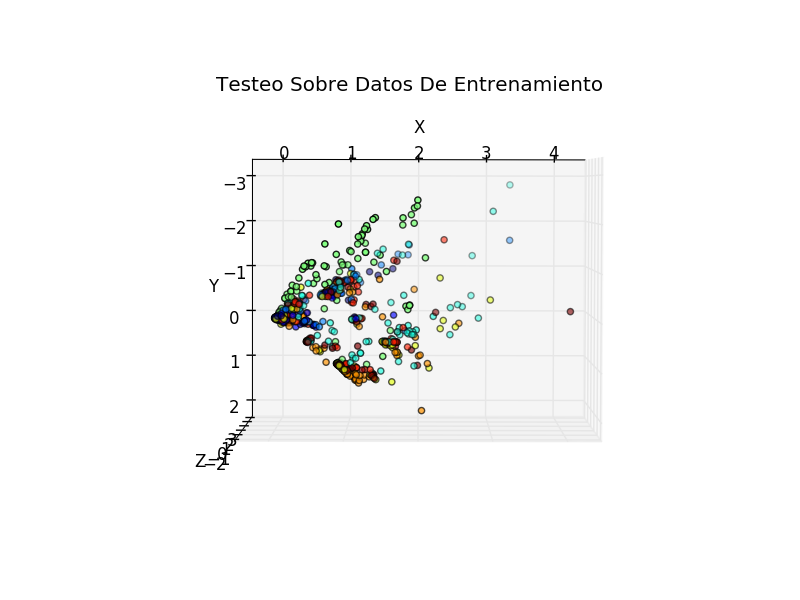
\includegraphics[width=.9\linewidth]{testeo_test_set_sanger/entrenamiento12.png}
  \captionof{figure}{Datos Entrenamiento}
  \label{fig:test1}
\end{minipage}%
\hspace{-3cm}
\begin{minipage}{.7\textwidth}
  \centering
  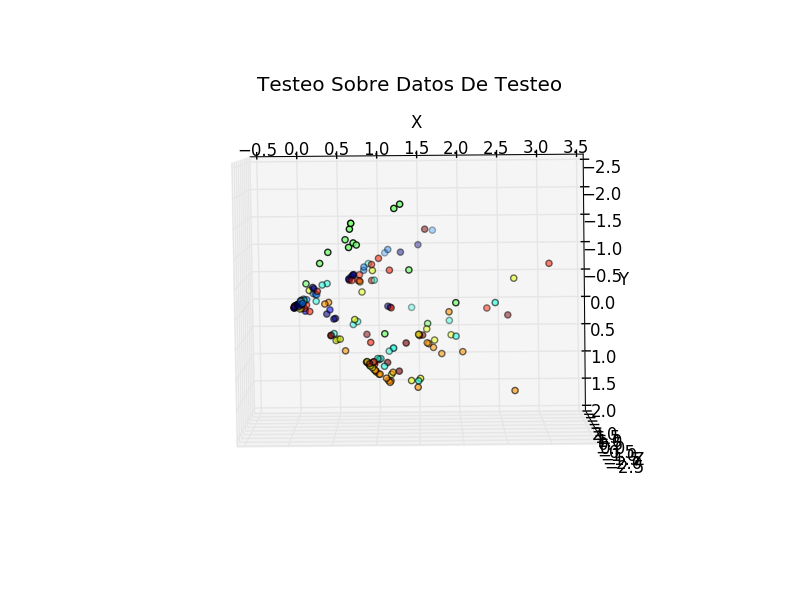
\includegraphics[width=.9\linewidth]{testeo_test_set_sanger/test_12.png}
  \captionof{figure}{Datos Testeo}
  \label{fig:test2}
\end{minipage}
\captionof{figure}{sanger}
\end{figure}

Si bien en algos algoritmos pueden verse puntos que estan fuera del area esperada (por ejemplo en oja, abajo a la izquierda puede verse un punto rojo), concideramos que esto puede deberse al ruido que poseen de manera hinerita los datos. Como una posible solución a los datos, podriían preprocesarse para intentar quitar outliers que empeoren los resultados de los algoritmos haciendolos aprender el ruido de los datos.

\pagebreak

\subsection{Mapeo de Características}

En este apartado construiremos un modelo de mapeo de caracteristicas auto-organizado con la intención de clasificar los documentos en un arreglo de dos dimenciones. Para ello utilizaremos el algoritmo de Kohonen sobre los datos de entrenamiento y una vez que la red haya convergido, intentaremos darle sentido a los resultados.

\subsubsection{Implementación}

El algoritmo basico utilizado será el visto en clases, que basicamente se divide en:

\begin{algorithm}
\begin{algorithmic}[1]\parskip=1mm
 \caption{ Activación(x)}
 \STATE{$\tilde y = \norm{x^T -MatrizDePesos}$}
 \STATE{$y = (\tilde y == min(\tilde y))*1.0$}
 \STATE{retornar $y$}
\end{algorithmic}
\end{algorithm}

\begin{algorithm}
\begin{algorithmic}[1]\parskip=1mm
 \caption{ correccion(x,y)}
 \STATE{$j^* = np.nonzero(y)$}
 \STATE{$D = \Delta(j^*,epoca)$}
 \STATE{$\Delta pesos = learning_rate(epoca).D(x^T-self.weights)$}
 \STATE{$MatrizDePesos = MatrizDePesos + \Delta pesos$}
\end{algorithmic}
\end{algorithm}

\begin{algorithm}
\begin{algorithmic}[1]\parskip=1mm
 \caption{ entrenamiento()}
 \STATE{Para cada instancia x de entrenamiento:}
 \STATE{\quad $y = Activacion(x)$}
 \STATE{\quad $correccion(x,y)$}
\end{algorithmic}
\end{algorithm}

El learning rate comenzará con un valor inicial relativamente alto e irá decreciendo en cada iteración (sin alcanzar al valor cero nunca).

Nuevamente este codigo resulta facilmente adaptable a python.

\subsubsection{Convergencia Kohonen}

Para esta experimentación utilizamos un learning rate adaptativo igual a $learning_rate_inicial / (1 + epocas * learning_rate_proporcional * learning_rate_inicial)$, con $learning_rate_inicial=0.7$  y $learning_rate_proporcional=0.5$

Abajo mostramos la convergencia a priori del algoritmo:

\begin{figure}[h!]
\centering
\begin{minipage}{.15\textwidth}
  \centering
  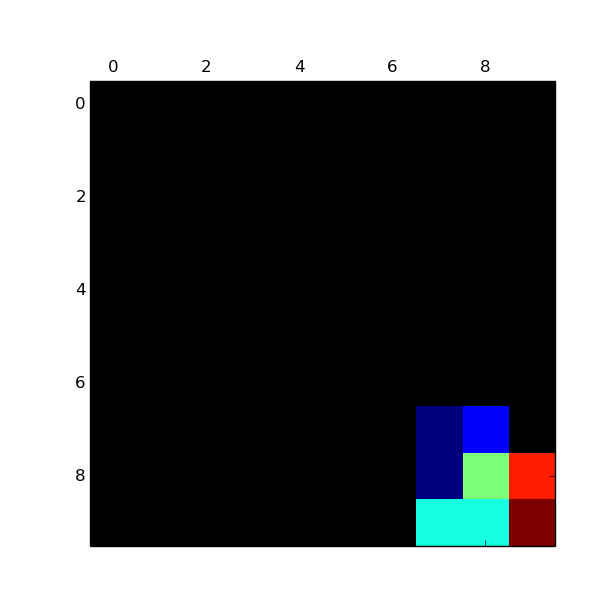
\includegraphics[width=.9\linewidth]{img/convergencia_kohonen/entrenamiento_0.png}
  \captionof{figure}{0\%}
  \label{fig:test1}
\end{minipage}%
\begin{minipage}{.15\textwidth}
  \centering
  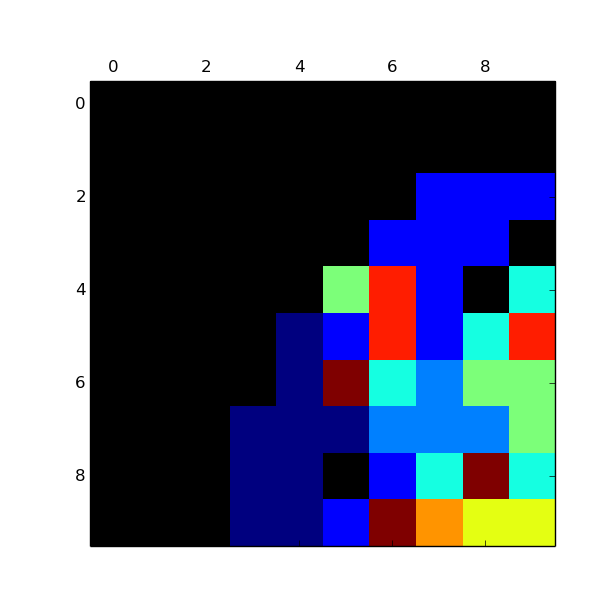
\includegraphics[width=.9\linewidth]{img/convergencia_kohonen/entrenamiento_25.png}
  \captionof{figure}{25\%}
  \label{fig:test2}
\end{minipage}
\begin{minipage}{.15\textwidth}
  \centering
  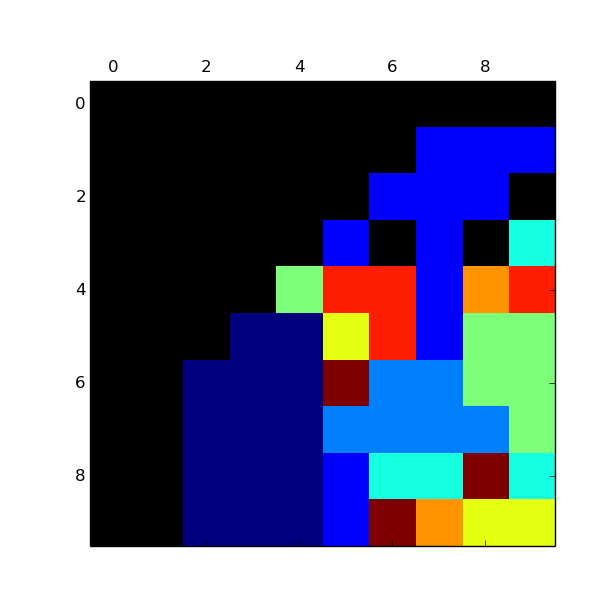
\includegraphics[width=.9\linewidth]{img/convergencia_kohonen/entrenamiento_50.png}
  \captionof{figure}{50\%}
  \label{fig:test2}
\end{minipage}
\begin{minipage}{.15\textwidth}
  \centering
  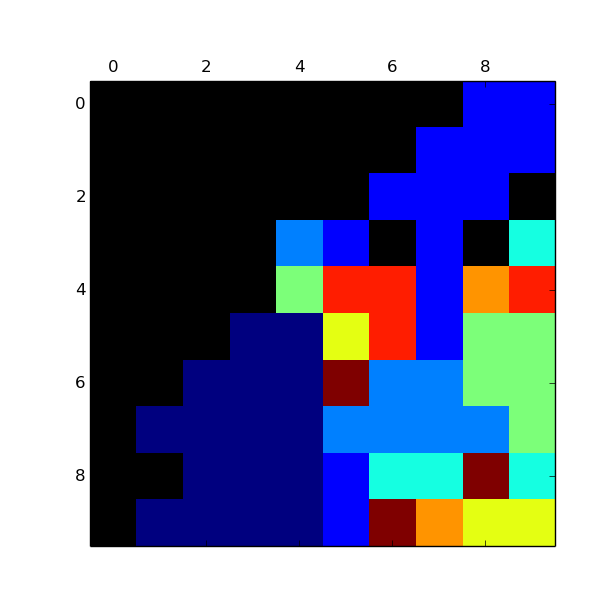
\includegraphics[width=.9\linewidth]{img/convergencia_kohonen/entrenamiento_75.png}
  \captionof{figure}{75\%}
  \label{fig:test2}
\end{minipage}
\begin{minipage}{.15\textwidth}
  \centering
  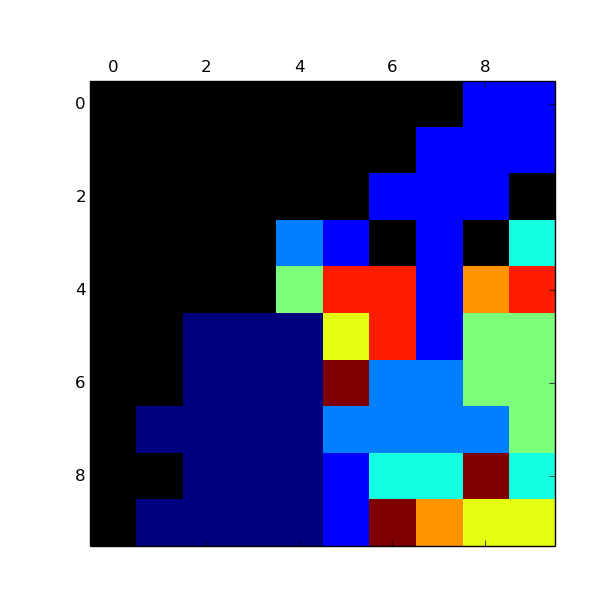
\includegraphics[width=.9\linewidth]{img/convergencia_kohonen/entrenamiento_100.png}
  \captionof{figure}{100\%}
  \label{fig:test2}
\end{minipage}
\end{figure}

Aqui puede verse de manera bastante clara como se van organizando las diferentes categorías.